\chapter{Experimental Methodology}\label{ch:method}

\section{Evidence categories}

Results in this project fall into five categories. They are labelled separately throughout
because they are not interchangeable, and a reader is entitled to know which kind of claim any
particular number is.

\begin{longtable}{@{}p{0.19\textwidth}p{0.36\textwidth}p{0.38\textwidth}@{}}
\toprule
\textbf{Category} & \textbf{What it is} & \textbf{What it does \emph{not} transfer to} \\
\midrule
\endhead
Formal & Exhaustive model checking of the TLA+ specifications & Holds of the \emph{model}. It
transfers to the implementation only as far as the trace-conformance check establishes. \\
Simulation & The unmodified firmware logic driven by a seeded harness on a host. E1--E5. &
No radio, no true parallelism, no CPU contention. Carries \textbf{no} timing information. \\
Testbed measurement & Observation of a live external system. E6 only: eight scenarios against
a running Mosquitto 2.0.18. & Ran on loopback with a private certificate authority, not in a
deployed wireless network. \\
Analytical & Follows from the construction rather than from running anything: the $2^{-128}$
forgery probability, the zero blocking term, the response-time decomposition. & Analytical
bounds say nothing about the residual hardware term. \\
Corpus study & Static analysis over 135 commit-pinned open-source projects. E7. & The corpus
is biased by construction; the result is an existence claim, never a prevalence estimate. \\
\bottomrule
\end{longtable}

No result in this project is a physical measurement of the running device. The single exception
is the build cost in Table~\ref{tab:rep-build}, measured by a real compiler, which describes the
binary rather than the device executing it.

\section{Hypotheses}

Two hypotheses were stated before the experiments were designed.

\begin{description}[leftmargin=2.4em,itemsep=5pt]
  \item[H1 (logical isolation).] No control- or data-flow dependency exists by which network
        activity can block, delay or corrupt the safety path.
        \emph{Status: tested, and supported} — by exhaustive model checking of the
        \code{Isolation} specification and by 19,529 trace-conformance checks.
  \item[H2 (timing isolation).] $F_{\Lambda} \stackrel{d}{=} F_{0}$ for radio-layer load
        $\Lambda$ across the operating range.
        \emph{Status: \textbf{requires hardware; not tested here}.} The protocol that would
        test it is Appendix~\ref{app:hardware}.
\end{description}

H2 is the hypothesis that motivated the project, and it is the one that remains open. Nothing in
Chapter~\ref{ch:results} should be read as evidence for or against it.

\section{Determinism and reproduction}

Every simulated experiment is seeded, and every seed is recorded with the result. The campaign
uses seed 1000, the ablation seed 2000, and the fuzzer seed 7. Re-running any harness from a
clean checkout regenerates byte-identical records.

Three further measures were taken because reproducibility claims are easy to make and hard to
honour:

\begin{itemize}[leftmargin=1.6em,itemsep=4pt]
  \item \textbf{A process per trial.} The campaign harness forks for each trial, so no state
        can leak between trials through a static variable or an allocator.
  \item \textbf{Standard library only for statistics.} Fisher's exact test and the Wilson
        interval are implemented in the repository. No external statistical package can alter a
        reported value, and the Wilson implementation is duplicated independently in two scripts
        that are checked for agreement.
  \item \textbf{Figures validated against raw records.}
        \code{experiments/validate\_figures.py} recomputes every plotted value from
        \code{ablation.jsonl} rather than from the derived summary, so a figure agreeing with a
        stale aggregate cannot pass.
\end{itemize}

\section{Metrics}

\begin{longtable}{@{}p{0.26\textwidth}p{0.66\textwidth}@{}}
\toprule
\textbf{Metric} & \textbf{Definition} \\
\midrule
\endhead
Safety latency & Simulated milliseconds from confirmed sensor assertion to entry-delay entry.
\emph{Simulated, and therefore constant by construction.} \\
Command availability & Trials in which a legitimate command issued during the flood took
effect \\
Integrity failure & Trials in which an adversary's message caused a state change \\
Replay defeat & Trials in which the adversary obtained an accepted command using only captured
or forged material \\
Invariant violation & Trials violating any safety invariant \\
Accepted fuzz input & Inputs changing state or advancing the counter without a valid tag \\
False-positive rate & Benign runs in which the detector reported at least once \\
Detection latency & Simulated milliseconds from attack onset to first detector report \\
\bottomrule
\end{longtable}

\section{The experiments}

\subsection{E1 and E2: the adversarial campaign}

\textbf{Objective.} Determine whether a remote adversary can change the alarm's state or
prevent a legitimate operator command from taking effect, with and without command
authentication.

\textbf{Design.} 3,000 trials per build across six attack rates from 0 to 20,000 messages per
second. The independent variables are the build configuration (baseline or hardened) and the
attack rate; the dependent variables are integrity failure, command availability and invariant
violation. The rate-0 arms are the controls.

\textbf{Harness.} \code{experiments/campaign.cpp}, one \code{fork()} per trial, seed 1000.

\subsection{E3: the command-path ablation}

\textbf{Objective.} Determine which command-path defence preserves the safety function,
operator availability and replay resistance — treating the three as separate properties rather
than assuming they rise and fall together.

\textbf{Design.} Twelve configurations, 300 trials each, 3,600 trials in total, all on identical
seeds. The configurations are not variations on a theme: six are command-path designs and six
are credential-compromise scenarios, indexed by which secret the adversary holds.

\begin{longtable}{@{}p{0.27\textwidth}p{0.63\textwidth}@{}}
\toprule
\textbf{Mode} & \textbf{What it models} \\
\midrule
\endhead
\code{none}                    & No command defence at all \\
\code{ratelimit}               & Token-bucket rate limiting \\
\code{token}                   & A static shared token \\
\code{transport}               & TLS with credentials held securely \\
\code{transport\_leaked}       & TLS with one credential leaked \\
\code{hmac}                    & HMAC-SHA256 over a monotonic counter \\
\code{acl\_shared\_leaked}     & Access control list, one shared credential leaked \\
\code{acl\_operator\_leaked}   & Access control list, controller credential leaked \\
\code{acl\_device\_leaked}     & Access control list, device credential leaked \\
\code{hmac\_keyleaked}         & HMAC with the command key compromised \\
\code{acl\_hmac\_devicedump}   & All three layers, device credential + key (flash dump) \\
\code{acl\_hmac\_controllerdump} & All three layers, controller credential + key \\
\bottomrule
\end{longtable}

\textbf{Harness.} \code{experiments/ablation.cpp}, seed 2000. Broker admission and access
control are modelled in \code{deliverGuarded}/\code{admit}; the device-side checks are the
firmware's own \code{handleCommands}.

\textbf{Availability measurement.} Operator availability is measured over \emph{five} attempts
per trial at 200\,ms intervals, not one. This matters, and the reason is given in
Section~\ref{sec:method-defects}.

\subsection{E4: host-build fuzzing}

\textbf{Objective.} Determine whether the command parser mishandles malformed input.

\textbf{Design.} 3,000,000 iterations across six input classes, seed 7, under both
AddressSanitizer and UndefinedBehaviorSanitizer.

\textbf{Scope, stated plainly.} The fuzzer exercises the parser \emph{compiled for the host},
not the binary running on the device. That is what makes the sanitizers usable and it is equally
the limit of the result: it says nothing about faults depending on the Xtensa toolchain's code
generation, on the real memory map, or on the radio driver's own parsing. This is host fuzzing,
not firmware rehosting, and the two are not interchangeable \cite{pemu2025}.

\subsection{E5: detector parameter sensitivity}

\textbf{Objective.} Determine whether the deauthentication detector's shipped threshold and
window are appropriate.

\textbf{Design.} A 180-cell grid over threshold and window values, with benign and attack
traffic classes. The dependent variables are the false-positive rate and the detection latency.

This experiment produced a correction rather than a confirmation, which is why it is reported
rather than dropped.

\subsection{E6: access control against a live broker}

\textbf{Objective.} Determine whether the access-control results modelled in E3 hold against
real broker software.

\textbf{Design.} Eight scenarios against a live Mosquitto 2.0.18 instance with TLS 1.2, a
private certificate authority, a \code{mosquitto\_passwd} file and a deny-by-default
\code{acl\_file}. Two access-control variants are tested — per-client and single-shared-credential
— each with its own legitimate control.

\textbf{The critical methodological decision.} Every verdict is decided by whether a subscriber
holding the device identity \emph{actually received} the message, never by PUBACK. MQTT 3.1.1
has no return code meaning ``refused by policy'', so a broker that discards a publication for
violating the access control list still acknowledges a QoS~1 publish. The summary deliberately
prints the PUBACK column in order to show that it is uninformative.

\textbf{Limitation.} The broker ran on loopback with a private certificate authority, not in a
deployed wireless network.

\subsection{E7: the open-source corpus study}

\textbf{Objective.} Determine whether the configuration defect found in this system appears in
comparable open-source projects.

\textbf{Design.} 135 projects selected by 22 fixed GitHub queries with a minimum of 3 stars and
a maximum size of 80\,MB, excluding archived repositories and forks. Every project is pinned to
a commit hash recorded in \code{commit\_shas.tsv}. Two static rules are applied: a precise guard
pattern (Rule~1) and a looser no-application-authentication heuristic (Rule~2).

\textbf{Controls.} Eight, including this project's \emph{own} pre-repair guard as a positive
control and its repaired guard as a negative control. The reason is given in
Section~\ref{sec:method-defects}.

\textbf{Bias, stated up front.} The corpus is biased by construction. Query selection, the star
threshold and the size cap all shape it. Whatever the result, it cannot support a prevalence
claim about the wider ecosystem.

\subsection{E8 and E9: conformance and model checking}

\textbf{E8, trace conformance.} The transition relation is parsed out of
\code{formal/AlarmFSM.tla} — rather than restated — and 19,529 firmware transitions observed
across three ablation modes are checked against it. A negative control asserts that a forbidden
\code{Disarmed} $\rightarrow$ \code{Alarm} transition \emph{is} rejected.

\textbf{E9, model checking.} Three TLC configurations: \code{AlarmFSM}, \code{Isolation}, and a
deliberately defective \code{AlarmFSM\_unsafe} which the runner requires to \emph{fail}.
Chapter~\ref{ch:formal} explains why the third exists.

\section{The experimental setup as a whole}

Figure~\ref{fig:setup} distinguishes what has been run from what has only been specified.

\begin{figure}[htbp]
\centering
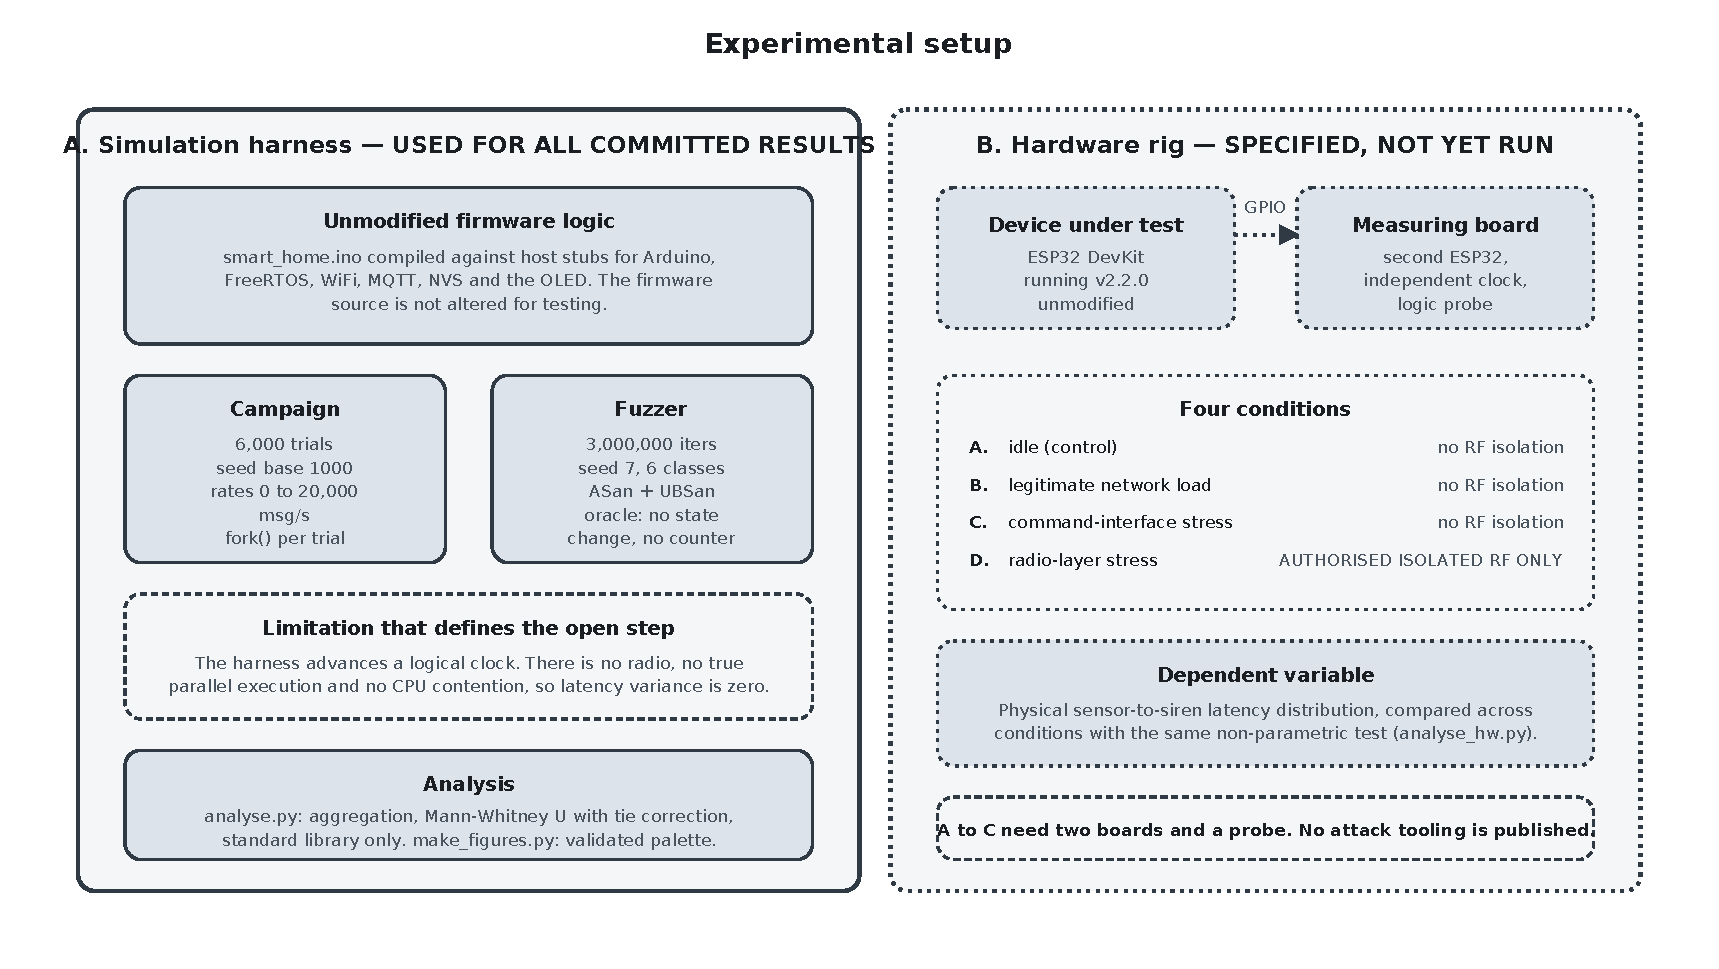
\includegraphics[width=\textwidth]{experimental_setup.pdf}
\caption[Experimental setup]{Experimental setup. Panel~A is everything that has been run: the
host simulation harness (E1--E5) and the real-broker testbed (E6), which is a live Mosquitto
instance and not a simulation. Panel~B is the hardware rig: specified, built as a protocol, and
\textbf{not run}. No number anywhere in this report comes from panel~B.}
\label{fig:setup}
\end{figure}

\section{Defects found in the measurement infrastructure}\label{sec:method-defects}

Four defects were found in the harnesses themselves during this work. Two of them produced
results that flattered the intended conclusion, which is precisely why they are reported here
rather than quietly corrected. A reader assessing the credibility of
Chapter~\ref{ch:results}'s numbers is entitled to know how the instrument was tested.

\begin{enumerate}[leftmargin=1.8em,itemsep=6pt]
  \item \textbf{Operator availability was unattributable.} The original measurement recorded
        whether a legitimate command took effect, but the adversary in the harness could also
        publish \code{ARM} — so an observed state change could not be attributed to the
        operator. Fixed by suppressing adversary \code{ARM} publications for the whole
        measurement prologue.
  \item \textbf{The first fix was itself wrong.} The quiet settling period introduced by that
        fix allowed the token bucket to refill before the measurement, so the rate limiter
        appeared more available than it is. Fixed by holding the suppression across the entire
        prologue rather than part of it.
  \item \textbf{A single-attempt measurement measured the wrong thing.} Availability recorded as
        one boolean per trial was in fact measuring the token bucket's \emph{phase} at the
        instant of the attempt, producing residues of 0.5, 0.9 and 0.995 rather than a rate.
        Fixed by measuring five attempts per trial at 200\,ms intervals, which is why the
        availability denominator is 1,250 and not 300.
  \item \textbf{A button hold shorter than the debounce window.} The harness held the simulated
        button for 40\,ms against a 40\,ms debounce threshold, so local arming was intermittent
        for reasons unrelated to the experiment. Fixed to 80\,ms.
\end{enumerate}

The campaign was re-run from scratch after these corrections, and every number in
Chapter~\ref{ch:results} comes from the corrected harness.

A fifth defect, in the corpus rule rather than the harness, is reported in
Section~\ref{sec:res-corpus}: the rule initially returned zero against this project's own
pre-repair guard, because the identifier it looked for appears there \emph{negated}. Until that
was found, the zero result was meaningless. The eight controls exist as a direct consequence.
